\chapter{Performance prediction through simulation: the HPL case}
\label{chapter:prediction}

The work presented in this chapter has been published at a conference\cite{cornebize:cluster19} and has been submitted
for publication in a journal. The content of this chapter is therefore a near-verbatim copy of these articles.

\section{High Performance Linpack}%
\label{sec:prediction:hpl}

    \subsection{The benchmark}%
    \label{sub:hpl:benchmark}

        \begin{figure}[ht]
            \newcommand{\mykwfn}[1]{{\textbf{\textsf{#1}}}}%
            \SetAlFnt{\textsf}%
            \SetKwSty{mykwfn}%
            \SetKw{KwStep}{step}%
            \centering
            \begin{minipage}[m]{0.5\linewidth}
                % \vspace{0.3cm} % ugly, could not align the drawing with the algorithm with minipages or tabular...
                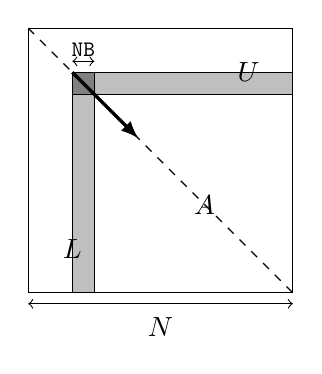
\begin{tikzpicture}[scale=0.28]
                    \draw (0, 0) -- (0, 12) -- (12, 12) -- (12, 0) -- cycle;
                    \foreach \i in {2}{
                        \draw [fill=lightgray] (\i, 0) -- (\i, 12-\i) -- (12, 12-\i) -- (12, 0) -- cycle;
                        \draw [fill=gray] (\i, 12-\i) -- (\i, 12-\i-1) -- (\i+1, 12-\i-1) -- (\i+1, 12-\i) -- cycle;
                        \draw[very thick, -latex] (\i,12-\i) -- (\i+2,12-\i-2);
                        \draw[<->] (\i, 12-\i+0.5) -- (\i+1, 12-\i+0.5) node [pos=0.5, yshift=+0.15cm] {\scalebox{.8}{\texttt{NB}}};
                    }
                    \foreach \i in {3}{
                        \draw [fill=white] (\i, 0) -- (\i, 12-\i) -- (12, 12-\i) -- (12, 0) -- cycle;
                        \draw (\i,12-\i) -- (\i,0);
                        \draw[very thick, -latex] (\i,12-\i) -- (\i+2,12-\i-2);
                    }
                    \draw[dashed] (0, 12) -- (12, 0);
                    \node(L) at (2, 2) {\ensuremath{\boldsymbol{L}}};
                    \node(U) at (10, 10) {\ensuremath{\boldsymbol{U}}};
                    \node(A) at (8, 4) {\ensuremath{\boldsymbol{A}}};
                    \draw[<->] (0, -0.5) -- (12, -0.5) node [pos=0.5, yshift=-0.3cm] {$N$};
                \end{tikzpicture}
            \end{minipage}%
            \begin{minipage}[m]{0.5\linewidth}
                \begin{algorithm}[H]
                    allocate and initialize $A$\;
                    \For{$k=N$ \KwTo $0$ \KwStep \texttt{NB}}{
                        allocate the panel\;
                        factor the panel\;
                        broadcast the panel\;
                        update the sub-matrix;
                    }
                \end{algorithm}
                \vspace{1em}
            \end{minipage}\vspace{-.5em}
            \caption{Overview of High Performance Linpack}\vspace{-1.5em}
            \label{fig:hpl_overview}
        \end{figure}

        In this work, we use the freely-available reference-implementation of HPL\cite{hpl}, which relies on MPI.  HPL
        implements a matrix factorization based on a right-looking variant of the LU factorization with row partial pivoting
        and allows multiple look-ahead depths. The principle of the factorization is depicted in
        Figure\ref{fig:hpl_overview}. It consists of a series of panel factorizations followed by an update of the trailing
        sub-matrix.  HPL uses a two-dimensional block-cyclic data distribution of $A$ and implements several custom MPI
        collective communication algorithms to efficiently overlap communications with computations.
        The main parameters of HPL are:
        \begin{itemize}
            \item \texttt{N} is the order of the square matrix $A$.
            \item \texttt{NB} is the \emph{blocking factor}, \ie the granularity at which HPL operates when panels are
                distributed or worked on.
            \item \texttt{P} and \texttt{Q} denote the number of process rows and the number of process columns,
                respectively.
            \item \texttt{RFACT} determines the panel factorization algorithm. Possible values are Crout, left- or
                right-looking.
            \item \texttt{SWAP} specifies the swapping algorithm used while pivoting. Two algorithms are available: one
                based on \emph{binary exchange} (along a virtual tree topology) and the other one based on a
                \emph{spread-and-roll} (with a higher number of parallel communications). HPL also provides a panel-size
                threshold triggering a switch from one variant to the other.
            \item \texttt{BCAST} sets the algorithm used to broadcast a panel of columns over the process columns. Legacy
                versions of the MPI standard only supported non-blocking point-to-point communications, which is why HPL
                ships with in total 6 self-implemented variants to overlap the time spent waiting for an incoming panel with
                updates to the trailing matrix: \texttt{ring}, \texttt{ring-modified}, \texttt{2-ring},
                \texttt{2-ring-modified}, \texttt{long}, and \texttt{long-modified}. The \texttt{modified} versions
                guarantee that the process right after the root (\ie the process that will become the root in the next
                iteration) receives data first and does not further participate in the broadcast. This process can thereby
                start working on the panel as soon as possible. The \texttt{ring} and \texttt{2-ring} versions each
                broadcast along the corresponding virtual topologies while the \texttt{long} version is a \emph{spread and
                roll} algorithm where messages are chopped into \texttt{Q} pieces. This generally leads to better bandwidth
                exploitation. The \texttt{ring} and \texttt{2-ring} variants rely on \texttt{MPI\_Iprobe}, meaning they
                return control if no message has been fully received yet, hence facilitating partial overlap of
                communication with computations.  In HPL 2.1 and 2.2, this capability has been deactivated for the
                \texttt{long} and \texttt{long-modified} algorithms. A comment in the source code states that some machines
                apparently get stuck when there are too many ongoing messages.
            \item \texttt{DEPTH} controls how many iterations of the outer loop can overlap with each other.
        \end{itemize}

        The sequential complexity of this factorization is \[\mathrm{flop}(N) = \frac{2}{3}N^3 + 2N^2 + \O(N)\] where $N$ is
        the order of the matrix to factorize. The time complexity can be approximated by \[T(N) \approx
        \frac{\left(\frac{2}{3}N^3 + 2N^2\right)}{P\cdot{}Q\cdot{}w} + \Theta((P+Q)\cdot{}N^2)\] where $w$ is the flop rate
        of a single node and the second term corresponds to the communication overhead which is influenced by the network
        capacity and the previously listed parameters (\texttt{RFACT}, \texttt{SWAP}, \texttt{BCAST},
        \texttt{DEPTH}, \ldots) and is very difficult to predict.

    \subsection{Typical runs on a supercomputer}%
    \label{sub:hpl:typical_runs}

        Although the TOP500 reports precise information about the core count,
        the peak performance and the effective performance, it provides almost
        no information on how (software versions, HPL parameters, etc.) this
        performance was achieved. Some colleagues agreed to provide us with
        the HPL configuration they used and the output they submitted for
        ranking (see Table\ref{fig:typical_run}).
        In June 2013, the Stampede supercomputer at TACC was ranked
        6th in the TOP500 by achieving \NSI{5168.1}{\tera\flops}. In November
        2017, the Theta supercomputer at ANL was ranked 18th with a performance of \NSI{5884.6}{\tera\flops}
        but required a 28-hour run on the
        whole machine. Finally, we ran HPL ourselves on a Grid'5000 cluster
        named Dahu whose software stack could be fully controlled.

        \begin{table}[hb]
            \caption{Typical runs of HPL}
            \label{fig:typical_run}
            \scalebox{.9}{\begin{tabular}{l|lll}
                \multicolumn{1}{l|}{} & Stampede@TACC & Theta@ANL & Dahu@G5K\\
                \hline
                \texttt{Rpeak}     & \NSI{8520.1}{\tera\flops} & \NSI{9627.2}{\tera\flops} & \NSI{62.26}{\tera\flops}              \\
                $N$         & \Num{3875000}                & \Num{8360352}                & \Num{500000}            \\
                \texttt{NB}        & \Num{1024}                    & 336                      & 128                \\
                $P\times Q$             & 77$\times$78                  & 32$\times$101                 & 32$\times$32            \\
                \texttt{RFACT}     & Crout                    & Left                     & Right              \\
                \texttt{SWAP}      & Binary-exch.             & Binary-exch.             & Binary-exch.       \\
                \texttt{BCAST}     & Long modified            & 2 Ring modified          & 2 Ring             \\
                \texttt{DEPTH}     & 0                        & 0                        & 1                  \\
                \hline
                \texttt{Rmax}      & \NSI{5168.1}{\tera\flops} & \NSI{5884.6}{\tera\flops} & \NSI{24.55}{\tera\flops}              \\
                Duration   & 2 hours                  & 28 hours                 & 1 hour             \\
                Memory    & \NSI{120}{\tera\byte}     & \NSI{559}{\tera\byte}     & \NSI{2}{\tera\byte} \\
                MPI ranks & 1/node                & 1/node                   & 1/core             \\
            \end{tabular}}
        \end{table}


        The performance typically achieved by supercomputers (\texttt{Rmax}) needs to be compared to the much larger
        peak performance (\texttt{Rpeak}). This difference can be attributed to the node usage, to the MPI library, to
        the network topology that may be unable to deal with the intense communication workload, to load imbalance among
        nodes (\eg due to a defect, system noise, \ldots), to the algorithmic structure of HPL, etc. All these factors
        make it difficult to know precisely what performance to expect without running the application at scale.  It is
        clear that due to the level of complexity of both HPL and the underlying hardware, simple performance models
        (analytic expressions based on $N, P, Q$ and estimations of platform characteristics) may be able to provide
        trends but can by no means accurately predict the performance for each configuration (\eg consider the exact
        effect of HPL's six different broadcast algorithms on network contention). Additionally, these expressions do
        not allow engineers to improve the performance through actively identifying performance bottlenecks.  For
        complex optimizations such as partially non-blocking collective communication algorithms intertwined with
        computations, a very faithful modeling of both the application and the platform is required. One goal of this
        thesis was to simulate systems at the scale of Stampede. Given the scale of this scenario (3,785~steps on
        6,006 nodes in two hours), detailed simulations quickly become intractable without significant effort.



\section{Simgrid/SMPI and the other simulators}%
\label{sec:prediction:simgrid}

    some text...

\section{Emulating HPL at large scale}%
\label{sec:prediction:emulation}

    some text...

\section{Modeling HPL kernels and communications}%
\label{sec:prediction:modeling}

    some text...

\section{Validation}%
\label{sec:prediction:validation}

    some text...

\section{Sensibility analysis}%
\label{sec:prediction:sensibility}

    some text...
